% Source PDF page 127 (printed p. 113)
\section*{习题}
\addcontentsline{toc}{section}{习题}
\subsection*{凸性的定义}
\paragraph{3.1}设 $f:\R\to\R$ 凸，$a,b\in\dom f$ 且 $a<b$。
\begin{enumerate}[label=(\alph*)]
\item 证明，对所有 $x\in[a,b]$，有
\[f(x)\leq\frac{b-x}{b-a}f(a)+\frac{x-a}{b-a}f(b).\]
\item 证明，对所有 $x\in(a,b)$，有
\[\frac{f(x)-f(a)}{x-a}\leq\frac{f(b)-f(a)}{b-a}\leq\frac{f(b)-f(x)}{b-x}.\]
画出说明这一不等式的示意图。
\item 设 $f$ 可微。利用(b)证明
\[f'(a)\leq\frac{f(b)-f(a)}{b-a}\leq f'(b).\]
这些不等式也可由式(3.2)得到：
\[f(b)\geq f(a)+f'(a)(b-a),\qquad f(a)\geq f(b)+f'(b)(a-b).\]
\item 设 $f$ 二次可微。利用(c)证明 $f''(a)\geq0$、$f''(b)\geq0$。
\end{enumerate}
\paragraph{3.2}\textit{凸函数、凹函数、拟凸函数与拟凹函数的水平集。}下图给出函数 $f$ 的几个水平集。标为1的曲线表示 $\{x\mid f(x)=1\}$，其他类似。
\begin{center}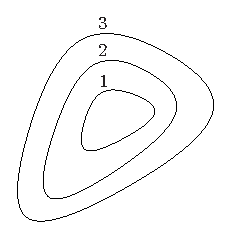
\includegraphics[width=.28\textwidth]{figures/ch03-ex127a.pdf}\end{center}
$f$ 是否可能凸、凹、拟凸或拟凹？说明理由。对下面的等高线重复上述问题。
\begin{center}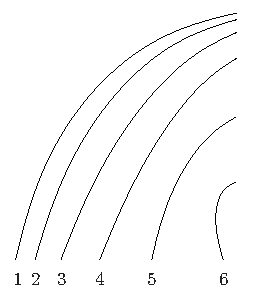
\includegraphics[width=.28\textwidth]{figures/ch03-ex127b.pdf}\end{center}
% Source PDF page 128 (printed p. 114)
\paragraph{3.3}\textit{递增凸函数的反函数。}设 $f:\R\to\R$ 在定义域 $(a,b)$ 上递增且凸。用 $g$ 表示它的反函数，即定义域为 $(f(a),f(b))$ 且对 $a<x<b$ 满足 $g(f(x))=x$ 的函数。关于 $g$ 的凸性或凹性，可以得到什么结论？
\paragraph{3.4}[RV73，第15页] 证明，连续函数 $f:\R^n\to\R$ 凸，当且仅当它在每条线段上的平均值不超过两个端点函数值的平均值：对任意 $x,y\in\R^n$，
\[\int_0^1 f(x+\lambda(y-x))\,d\lambda\leq\frac{f(x)+f(y)}2.\]
\paragraph{3.5}[RV73，第22页] \textit{凸函数的累积平均。}设 $f:\R\to\R$ 凸，$\R_+\subseteq\dom f$。证明，它的累积平均
\[F(x)=\frac1x\int_0^x f(t)\,dt,\qquad\dom F=\R_{++}\]
凸。\textit{提示：}对每个 $s$，$f(sx)$ 关于 $x$ 凸，因此 $\int_0^1 f(sx)\,ds$ 凸。
\paragraph{3.6}\textit{函数与上图。}函数的上图何时为半空间？何时为凸锥？何时为多面体？
\paragraph{3.7}设 $f:\R^n\to\R$ 凸，$\dom f=\R^n$，且在 $\R^n$ 上有上界。证明 $f$ 为常数。
\paragraph{3.8}\textit{凸性的二阶条件。}证明，二次可微函数 $f$ 凸，当且仅当其定义域凸，且对所有 $x\in\dom f$ 有 $\nabla^2f(x)\succeq0$。\textit{提示：}先考虑 $f:\R\to\R$。可以使用凸性的一阶条件，其证明见原书第70页。
\paragraph{3.9}\textit{仿射集上凸性的二阶条件。}设 $F\in\R^{n\times m}$、$\widehat x\in\R^n$。$f:\R^n\to\R$ 在仿射集 $\{Fz+\widehat x\mid z\in\R^m\}$ 上的限制定义为 $\widetilde f:\R^m\to\R$，其中
\[\widetilde f(z)=f(Fz+\widehat x),\qquad\dom\widetilde f=\{z\mid Fz+\widehat x\in\dom f\}.\]
设 $f$ 二次可微，且定义域凸。
\begin{enumerate}[label=(\alph*)]
\item 证明，$\widetilde f$ 凸，当且仅当对所有 $z\in\dom\widetilde f$ 有
\[F^\T\nabla^2f(Fz+\widehat x)F\succeq0.\]
\item 设 $A\in\R^{p\times n}$ 的零空间等于 $F$ 的值域，即 $AF=0$ 且 $\rank A=n-\rank F$。证明，若对所有 $z\in\dom\widetilde f$，存在 $\lambda\in\R$ 使
\[\nabla^2f(Fz+\widehat x)+\lambda A^\T A\succeq0,\]
则 $\widetilde f$ 凸。

\textit{提示：}使用如下结论：若 $B\in\mathbb S^n$、$A\in\R^{p\times n}$，并存在 $\lambda$ 使 $B+\lambda A^\T A\succeq0$，则对所有 $x\in\mathcal N(A)$ 有 $x^\T Bx\geq0$。
\end{enumerate}
\paragraph{3.10}\textit{Jensen 不等式的推广。}Jensen 不等式的一种解释是随机化或抖动会带来损失，即提高凸函数值的平均值：若 $f$ 凸、$v$ 为零均值随机变量，则 $\E f(x_0+v)\geq f(x_0)$。这引出如下猜想：若 $f$ 凸，则 $v$ 的方差越大，$\E f(x_0+v)$ 越大。
\begin{enumerate}[label=(\alph*)]
\item 给出反例说明这一猜想不成立。找出零均值随机变量 $v,w$，满足 $\operatorname{var}(v)>\operatorname{var}(w)$，以及凸函数 $f$ 和点 $x_0$，使 $\E f(x_0+v)<\E f(x_0+w)$。
% Source PDF page 129 (printed p. 115)
\item 当 $v,w$ 互为缩放时，这个猜想成立。证明，若 $f$ 凸且 $v$ 零均值，则 $\E f(x_0+tv)$ 在 $t\geq0$ 上单调增加。
\end{enumerate}
\paragraph{3.11}\textit{单调映射。}若函数 $\psi:\R^n\to\R^n$ 对所有 $x,y\in\dom\psi$ 满足
\[(\psi(x)-\psi(y))^\T(x-y)\geq0,\]
则称它单调。（这里“单调”的定义不同于3.6.1节，两种定义都广泛使用。）设 $f:\R^n\to\R$ 为可微凸函数。证明其梯度 $\nabla f$ 单调。逆命题是否成立，即每个单调映射都是某个凸函数的梯度吗？
\paragraph{3.12}设 $f:\R^n\to\R$ 凸、$g:\R^n\to\R$ 凹，$\dom f=\dom g=\R^n$，且对所有 $x$ 有 $g(x)\leq f(x)$。证明，存在仿射函数 $h$，对所有 $x$ 有 $g(x)\leq h(x)\leq f(x)$。换句话说，若凹函数 $g$ 是凸函数 $f$ 的下估计，则能在两者之间放入一个仿射函数。
\paragraph{3.13}\textit{Kullback--Leibler 散度与信息不等式。}设 $D_{\mathrm{kl}}$ 为式(3.17)定义的 Kullback--Leibler 散度。证明信息不等式：对所有 $u,v\in\R_{++}^n$ 有 $D_{\mathrm{kl}}(u,v)\geq0$。并证明 $D_{\mathrm{kl}}(u,v)=0$ 当且仅当 $u=v$。

\textit{提示：}Kullback--Leibler 散度可以表示为
\[D_{\mathrm{kl}}(u,v)=f(u)-f(v)-\nabla f(v)^\T(u-v),\]
其中 $f(v)=\sum_{i=1}^n v_i\log v_i$ 为 $v$ 的负熵。
\paragraph{3.14}\textit{凸—凹函数与鞍点。}若对每个固定的 $x$，$f(x,z)$ 关于 $z$ 凹，且对每个固定的 $z$，$f(x,z)$ 关于 $x$ 凸，则称 $f:\R^n\times\R^m\to\R$ 为凸—凹函数。还要求其定义域具有乘积形式 $\dom f=A\times B$，其中 $A\subseteq\R^n$、$B\subseteq\R^m$ 均凸。
\begin{enumerate}[label=(\alph*)]
\item 用 Hessian $\nabla^2f(x,z)$ 给出二次可微函数 $f:\R^n\times\R^m\to\R$ 为凸—凹函数的二阶条件。
\item 设 $f:\R^n\times\R^m\to\R$ 凸—凹且可微，$\nabla f(\widetilde x,\widetilde z)=0$。证明鞍点性质：对所有 $x,z$ 有
\[f(\widetilde x,z)\leq f(\widetilde x,\widetilde z)\leq f(x,\widetilde z).\]
证明这蕴含 $f$ 满足强极大极小性质：
\[\sup_z\inf_x f(x,z)=\inf_x\sup_z f(x,z),\]
两者的共同值为 $f(\widetilde x,\widetilde z)$。
\item 现在设 $f:\R^n\times\R^m\to\R$ 可微，但不必凸—凹，并在 $\widetilde x,\widetilde z$ 处具有鞍点性质：
\[f(\widetilde x,z)\leq f(\widetilde x,\widetilde z)\leq f(x,\widetilde z)\qquad\text{对所有 }x,z.\]
证明 $\nabla f(\widetilde x,\widetilde z)=0$。
\end{enumerate}
\subsection*{例子}
\paragraph{3.15}\textit{一族凹效用函数。}对 $0<\alpha\leq1$，令
\[u_\alpha(x)=\frac{x^\alpha-1}{\alpha},\qquad\dom u_\alpha=\R_+.\]
另定义 $u_0(x)=\log x$，$\dom u_0=\R_{++}$。
\begin{enumerate}[label=(\alph*)]
\item 证明，对 $x>0$，$u_0(x)=\lim_{\alpha\to0}u_\alpha(x)$。
% Source PDF page 130 (printed p. 116)
\item 证明各 $u_\alpha$ 凹、单调增加，并且都满足 $u_\alpha(1)=0$。
\end{enumerate}
这些函数常用于经济学，描述某种数量的商品或金钱所带来的收益或效用。$u_\alpha$ 的凹性意味着边际效用，即商品增加固定数量所获得的效用增量，随商品数量增加而减少。换句话说，凹性描述了饱和效应。
\paragraph{3.16}判断下列各函数是否凸、凹、拟凸或拟凹。
\begin{enumerate}[label=(\alph*)]
\item $\R$ 上的 $f(x)=e^x-1$。
\item $\R_{++}^2$ 上的 $f(x_1,x_2)=x_1x_2$。
\item $\R_{++}^2$ 上的 $f(x_1,x_2)=1/(x_1x_2)$。
\item $\R_{++}^2$ 上的 $f(x_1,x_2)=x_1/x_2$。
\item $\R\times\R_{++}$ 上的 $f(x_1,x_2)=x_1^2/x_2$。
\item $\R_{++}^2$ 上的 $f(x_1,x_2)=x_1^\alpha x_2^{1-\alpha}$，其中 $0\leq\alpha\leq1$。
\end{enumerate}
\paragraph{3.17}设 $p<1$、$p\ne0$。证明，函数
\[f(x)=\left(\sum_{i=1}^n x_i^p\right)^{1/p},\qquad\dom f=\R_{++}^n\]
凹。这包括特例 $f(x)=(\sum_{i=1}^n x_i^{1/2})^2$ 以及调和平均 $f(x)=(\sum_{i=1}^n1/x_i)^{-1}$。
\textit{提示：}改写3.1.5节中指数和对数函数及几何平均的证明。
\paragraph{3.18}改写3.1.5节中行列式对数函数凹性的证明，得到以下结论。
\begin{enumerate}[label=(\alph*)]
\item $f(X)=\tr(X^{-1})$ 在 $\dom f=\mathbb S_{++}^n$ 上凸。
\item $f(X)=(\det X)^{1/n}$ 在 $\dom f=\mathbb S_{++}^n$ 上凹。
\end{enumerate}
\paragraph{3.19}\textit{非负加权和与积分。}
\begin{enumerate}[label=(\alph*)]
\item 证明，$f(x)=\sum_{i=1}^r\alpha_i x_{[i]}$ 是 $x$ 的凸函数，其中 $\alpha_1\geq\alpha_2\geq\cdots\geq\alpha_r\geq0$，$x_{[i]}$ 是 $x$ 的第 $i$ 大分量。可以使用 $f(x)=\sum_{i=1}^k x_{[i]}$ 在 $\R^n$ 上凸这一事实。
\item 设 $T(x,\omega)$ 为三角多项式
\[T(x,\omega)=x_1+x_2\cos\omega+x_3\cos2\omega+\cdots+x_n\cos(n-1)\omega.\]
证明函数
\[f(x)=-\int_0^{2\pi}\log T(x,\omega)\,d\omega\]
在 $\{x\in\R^n\mid T(x,\omega)>0,\ 0\leq\omega\leq2\pi\}$ 上凸。
\end{enumerate}
\paragraph{3.20}\textit{与仿射函数复合。}证明以下函数 $f:\R^n\to\R$ 凸。
\begin{enumerate}[label=(\alph*)]
\item $f(x)=\norm{Ax-b}$，其中 $A\in\R^{m\times n}$、$b\in\R^m$，$\norm{\cdot}$ 为 $\R^m$ 上的范数。
\item $f(x)=-(\det(A_0+x_1A_1+\cdots+x_nA_n))^{1/m}$，定义域为 $\{x\mid A_0+x_1A_1+\cdots+x_nA_n\succ0\}$，其中 $A_i\in\mathbb S^m$。
\item $f(X)=\tr(A_0+x_1A_1+\cdots+x_nA_n)^{-1}$，定义域为 $\{x\mid A_0+x_1A_1+\cdots+x_nA_n\succ0\}$，其中 $A_i\in\mathbb S^m$。使用 $\tr(X^{-1})$ 在 $\mathbb S_{++}^m$ 上凸的结论，见习题3.18。
\end{enumerate}
% Source PDF page 131 (printed p. 117)
\paragraph{3.21}\textit{逐点最大值与上确界。}证明下列函数 $f:\R^n\to\R$ 凸。
\begin{enumerate}[label=(\alph*)]
\item $f(x)=\max_{i=1,\ldots,k}\norm{A^{(i)}x-b^{(i)}}$，其中 $A^{(i)}\in\R^{m\times n}$、$b^{(i)}\in\R^m$，$\norm{\cdot}$ 为 $\R^m$ 上的范数。
\item $f(x)=\sum_{i=1}^r|x|_{[i]}$，定义在 $\R^n$ 上，其中 $|x|$ 为满足 $|x|_i=|x_i|$ 的向量，即对 $x$ 逐分量取绝对值，$|x|_{[i]}$ 为 $|x|$ 的第 $i$ 大分量。换句话说，$|x|_{[1]},|x|_{[2]},\ldots,|x|_{[n]}$ 是 $x$ 的各分量绝对值按非增顺序排列后的结果。
\end{enumerate}
\paragraph{3.22}\textit{复合规则。}证明以下函数凸。
\begin{enumerate}[label=(\alph*)]
\item $f(x)=-\log(-\log(\sum_{i=1}^m e^{a_i^\T x+b_i}))$，$\dom f=\{x\mid\sum_{i=1}^m e^{a_i^\T x+b_i}<1\}$。可以使用 $\log(\sum_{i=1}^n e^{y_i})$ 凸的结论。
\item $f(x,u,v)=-\sqrt{uv-x^\T x}$，$\dom f=\{(x,u,v)\mid uv>x^\T x,\ u,v>0\}$。使用 $x^\T x/u$ 在 $u>0$ 时关于 $(x,u)$ 凸，以及 $-\sqrt{x_1x_2}$ 在 $\R_{++}^2$ 上凸这两个结论。
\item $f(x,u,v)=-\log(uv-x^\T x)$，$\dom f=\{(x,u,v)\mid uv>x^\T x,\ u,v>0\}$。
\item $f(x,t)=-(t^p-\norm x_p^p)^{1/p}$，其中 $p>1$，$\dom f=\{(x,t)\mid t\geq\norm x_p\}$。可以使用 $\norm x_p^p/u^{p-1}$ 在 $u>0$ 时关于 $(x,u)$ 凸（见习题3.23），以及 $-x^{1/p}y^{1-1/p}$ 在 $\R_+^2$ 上凸（见习题3.16）的结论。
\item $f(x,t)=-\log(t^p-\norm x_p^p)$，其中 $p>1$，$\dom f=\{(x,t)\mid t>\norm x_p\}$。可以使用 $\norm x_p^p/u^{p-1}$ 在 $u>0$ 时关于 $(x,u)$ 凸的结论，见习题3.23。
\end{enumerate}
\paragraph{3.23}\textit{函数的透视。}
\begin{enumerate}[label=(\alph*)]
\item 证明，当 $p>1$ 时，
\[f(x,t)=\frac{|x_1|^p+\cdots+|x_n|^p}{t^{p-1}}=\frac{\norm x_p^p}{t^{p-1}}\]
在 $\{(x,t)\mid t>0\}$ 上凸。
\item 证明
\[f(x)=\frac{\norm{Ax+b}_2^2}{c^\T x+d}\]
在 $\{x\mid c^\T x+d>0\}$ 上凸，其中 $A\in\R^{m\times n}$、$b\in\R^m$、$c\in\R^n$、$d\in\R$。
\end{enumerate}
\paragraph{3.24}\textit{概率单纯形上的一些函数。}设实值随机变量 $x$ 取值于 $\{a_1,\ldots,a_n\}$，其中 $a_1<a_2<\cdots<a_n$，且 $\Prob(x=a_i)=p_i$，$i=1,\ldots,n$。对下列各个关于 $p$ 的函数，在概率单纯形 $\{p\in\R_+^n\mid\one^\T p=1\}$ 上判断它是否凸、凹、拟凸或拟凹。
\begin{enumerate}[label=(\alph*)]
\item $\E x$。
\item $\Prob(x\geq\alpha)$。
\item $\Prob(\alpha\leq x\leq\beta)$。
\item $\sum_{i=1}^n p_i\log p_i$，即分布的负熵。
\item $\operatorname{var}x=\E(x-\E x)^2$。
\item $\operatorname{quartile}(x)=\inf\{\beta\mid\Prob(x\leq\beta)\geq0.25\}$。
\item 概率至少为90\% 的最小集合 $A\subseteq\{a_1,\ldots,a_n\}$ 的基数。基数指 $A$ 中元素的个数。
\item 包含90\% 概率的最窄区间的宽度，即
\[\inf\{\beta-\alpha\mid\Prob(\alpha\leq x\leq\beta)\geq0.9\}.\]
\end{enumerate}
% Source PDF page 132 (printed p. 118)
\paragraph{3.25}\textit{分布之间的最大概率距离。}设 $p,q\in\R^n$ 表示 $\{1,\ldots,n\}$ 上的两个概率分布，即 $p,q\succeq0$、$\one^\T p=\one^\T q=1$。将它们之间的最大概率距离 $d_{\mathrm{mp}}(p,q)$ 定义为所有事件上 $p,q$ 所赋概率之差的绝对值的最大值：
\[d_{\mathrm{mp}}(p,q)=\max\{|\Prob(p,C)-\Prob(q,C)|\mid C\subseteq\{1,\ldots,n\}\}.\]
这里 $\Prob(p,C)$ 为分布 $p$ 下 $C$ 的概率，即 $\Prob(p,C)=\sum_{i\in C}p_i$。

求出 $d_{\mathrm{mp}}$ 的一个简单表达式，用 $\norm{p-q}_1=\sum_{i=1}^n|p_i-q_i|$ 表示，并证明 $d_{\mathrm{mp}}$ 是 $\R^n\times\R^n$ 上的凸函数。它的定义域为 $\{(p,q)\mid p,q\succeq0,\ \one^\T p=\one^\T q=1\}$，但可以自然地延拓到整个 $\R^n\times\R^n$。
\paragraph{3.26}\textit{更多特征值函数。}设 $\lambda_1(X)\geq\lambda_2(X)\geq\cdots\geq\lambda_n(X)$ 为矩阵 $X\in\mathbb S^n$ 的特征值。前面已经看到几个关于 $X$ 凸或凹的特征值函数。
\begin{itemize}
\item 最大特征值 $\lambda_1(X)$ 凸（例3.10）；最小特征值 $\lambda_n(X)$ 凹。
\item 特征值之和，即迹 $\tr X=\lambda_1(X)+\cdots+\lambda_n(X)$，线性。
\item 特征值倒数之和，即逆矩阵的迹 $\tr(X^{-1})=\sum_{i=1}^n1/\lambda_i(X)$，在 $\mathbb S_{++}^n$ 上凸（习题3.18）。
\item 特征值的几何平均 $(\det X)^{1/n}=(\prod_{i=1}^n\lambda_i(X))^{1/n}$，以及特征值乘积的对数 $\log\det X=\sum_{i=1}^n\log\lambda_i(X)$，在 $X\in\mathbb S_{++}^n$ 上凹（习题3.18及原书第74页）。
\end{itemize}
本题利用变分刻画研究更多的特征值函数。
\begin{enumerate}[label=(\alph*)]
\item \textit{最大的 $k$ 个特征值之和。}证明 $\sum_{i=1}^k\lambda_i(X)$ 在 $\mathbb S^n$ 上凸。
\textit{提示：}[HJ85，第191页] 使用变分刻画
\[\sum_{i=1}^k\lambda_i(X)=\sup\{\tr(V^\T XV)\mid V\in\R^{n\times k},\ V^\T V=I\}.\]
\item \textit{最小的 $k$ 个特征值的几何平均。}证明 $(\prod_{i=n-k+1}^n\lambda_i(X))^{1/k}$ 在 $\mathbb S_{++}^n$ 上凹。
\textit{提示：}[MO79，第513页] 对 $X\succ0$，
\[\left(\prod_{i=n-k+1}^n\lambda_i(X)\right)^{1/k}
 =\frac1k\inf\{\tr(V^\T XV)\mid V\in\R^{n\times k},\ \det V^\T V=1\}.\]
\item \textit{最小的 $k$ 个特征值乘积的对数。}证明 $\sum_{i=n-k+1}^n\log\lambda_i(X)$ 在 $\mathbb S_{++}^n$ 上凹。
\textit{提示：}[MO79，第513页] 对 $X\succ0$，
\[\prod_{i=n-k+1}^n\lambda_i(X)
 =\inf\left\{\prod_{i=1}^k(V^\T XV)_{ii}\ \middle|\ V\in\R^{n\times k},\ V^\T V=I\right\}.\]
\end{enumerate}
\paragraph{3.27}\textit{Cholesky 因子的对角元。}每个 $X\in\mathbb S_{++}^n$ 都有唯一 Cholesky 分解 $X=LL^\T$，其中 $L$ 为下三角矩阵且 $L_{ii}>0$。证明 $L_{ii}$ 是 $X$ 的凹函数，定义域为 $\mathbb S_{++}^n$。

\textit{提示：}$L_{ii}$ 可表示为 $L_{ii}=(w-z^\T Y^{-1}z)^{1/2}$，其中
\[\begin{bmatrix}Y&z\\z^\T&w\end{bmatrix}\]
是 $X$ 的前 $i\times i$ 主子矩阵。
% Source PDF page 133 (printed p. 119)
\subsection*{保持凸性的运算}
\paragraph{3.28}\textit{把凸函数表示成一族仿射函数的逐点上确界。}本题将原书第83页证明的结论推广到 $\dom f\ne\R^n$。设 $f:\R^n\to\R$ 凸。定义 $\widetilde f:\R^n\to\R$ 为 $f$ 的所有仿射全局下估计的逐点上确界：
\[\widetilde f(x)=\sup\{g(x)\mid g\text{ 仿射},\ g(z)\leq f(z)\text{ 对所有 }z\text{ 成立}\}.\]
\begin{enumerate}[label=(\alph*)]
\item 证明，对 $x\in\operatorname{int}\dom f$，$f(x)=\widetilde f(x)$。
\item 证明，若 $f$ 闭，即 $\epi f$ 为闭集（见A.3.3节），则 $f=\widetilde f$。
\end{enumerate}
\paragraph{3.29}\textit{分段线性凸函数的表示。}凸函数 $f:\R^n\to\R$、$\dom f=\R^n$，若存在 $\R^n$ 的划分
\[\R^n=X_1\cup X_2\cup\cdots\cup X_L,\]
其中 $\operatorname{int}X_i\ne\varnothing$，且 $i\ne j$ 时 $\operatorname{int}X_i\cap\operatorname{int}X_j=\varnothing$，并有一族仿射函数 $a_1^\T x+b_1,\ldots,a_L^\T x+b_L$，使得 $x\in X_i$ 时 $f(x)=a_i^\T x+b_i$，则称 $f$ 分段线性。

证明，此类函数具有形式 $f(x)=\max\{a_1^\T x+b_1,\ldots,a_L^\T x+b_L\}$。
\paragraph{3.30}\textit{函数的凸包或凸包络。}函数 $f:\R^n\to\R$ 的凸包或凸包络定义为
\[g(x)=\inf\{t\mid(x,t)\in\conv\epi f\}.\]
几何上，$g$ 的上图是 $f$ 上图的凸包。

证明，$g$ 是 $f$ 的最大凸下估计。也就是说，若 $h$ 凸且对所有 $x$ 有 $h(x)\leq f(x)$，则对所有 $x$ 都有 $h(x)\leq g(x)$。
\paragraph{3.31}[Roc70，第35页] \textit{最大的齐次下估计。}设 $f$ 为凸函数，定义
\[g(x)=\inf_{\alpha>0}\frac{f(\alpha x)}\alpha.\]
\begin{enumerate}[label=(\alph*)]
\item 证明 $g$ 齐次，即对所有 $t\geq0$ 有 $g(tx)=tg(x)$。
\item 证明 $g$ 为 $f$ 的最大齐次下估计：若 $h$ 齐次且对所有 $x$ 有 $h(x)\leq f(x)$，则对所有 $x$ 有 $h(x)\leq g(x)$。
\item 证明 $g$ 凸。
\end{enumerate}
\paragraph{3.32}\textit{凸函数的乘积与比值。}一般来说，两个凸函数的乘积或比值不凸。但对 $\R$ 上函数存在一些结论。证明以下命题。
\begin{enumerate}[label=(\alph*)]
\item 若 $f,g$ 是区间上的正凸函数，并且都单调不减或都单调不增，则 $fg$ 凸。
\item 若 $f,g$ 为正凹函数，其中一个单调不减，另一个单调不增，则 $fg$ 凹。
\item 若 $f$ 凸、单调不减且为正，$g$ 凹、单调不增且为正，则 $f/g$ 凸。
\end{enumerate}
\paragraph{3.33}\textit{透视定理的直接证明。}直接证明：按3.2.6节定义的凸函数 $f$ 的透视 $g$ 凸。证明 $\dom g$ 为凸集，且对 $(x,t),(y,s)\in\dom g$、$0\leq\theta\leq1$ 有
\[g(\theta x+(1-\theta)y,\theta t+(1-\theta)s)\leq\theta g(x,t)+(1-\theta)g(y,s).\]
\paragraph{3.34}\textit{Minkowski 函数。}凸集 $C$ 的 Minkowski 函数定义为
\[M_C(x)=\inf\{t>0\mid t^{-1}x\in C\}.\]
% Source PDF page 134 (printed p. 120)
\begin{enumerate}[label=(\alph*)]
\item 画图，从几何上说明怎样求 $M_C(x)$。
\item 证明 $M_C$ 齐次，即对 $\alpha\geq0$ 有 $M_C(\alpha x)=\alpha M_C(x)$。
\item $\dom M_C$ 是什么？
\item 证明 $M_C$ 为凸函数。
\item 再设 $C$ 闭、有界、对称（$x\in C$ 蕴含 $-x\in C$），并有非空内部。证明 $M_C$ 为范数。对应的单位球是什么？
\end{enumerate}
\paragraph{3.35}\textit{支撑函数运算。}回顾，集合 $C\subseteq\R^n$ 的支撑函数定义为 $S_C(y)=\sup\{y^\T x\mid x\in C\}$。原书第81页已证明 $S_C$ 凸。
\begin{enumerate}[label=(\alph*)]
\item 证明 $S_B=S_{\conv B}$。
\item 证明 $S_{A+B}=S_A+S_B$。
\item 证明 $S_{A\cup B}=\max\{S_A,S_B\}$。
\item 设 $B$ 闭且凸。证明，$A\subseteq B$ 当且仅当对所有 $y$ 有 $S_A(y)\leq S_B(y)$。
\end{enumerate}
\subsection*{共轭函数}
\paragraph{3.36}求下列函数的共轭。
\begin{enumerate}[label=(\alph*)]
\item \textit{最大值函数。}$\R^n$ 上的 $f(x)=\max_{i=1,\ldots,n}x_i$。
\item \textit{最大元素之和。}$\R^n$ 上的 $f(x)=\sum_{i=1}^r x_{[i]}$。
\item \textit{$\R$ 上的分段线性函数。}$\R$ 上的 $f(x)=\max_{i=1,\ldots,m}(a_ix+b_i)$。可以假设 $a_i$ 已按递增顺序排列，即 $a_1\leq\cdots\leq a_m$，且每个函数 $a_ix+b_i$ 都不冗余，即对每个 $k$ 至少存在一个 $x$ 使 $f(x)=a_kx+b_k$。
\item \textit{幂函数。}$\R_{++}$ 上的 $f(x)=x^p$，$p>1$。再对 $p<0$ 求解。
\item \textit{负几何平均。}$\R_{++}^n$ 上的 $f(x)=-(\prod x_i)^{1/n}$。
\item \textit{二阶锥的负广义对数。}$f(x,t)=-\log(t^2-x^\T x)$，定义在 $\{(x,t)\in\R^n\times\R\mid\norm x_2<t\}$ 上。
\end{enumerate}
\paragraph{3.37}证明，$f(X)=\tr(X^{-1})$、$\dom f=\mathbb S_{++}^n$ 的共轭为
\[f^*(Y)=-2\tr(-Y)^{1/2},\qquad\dom f^*=-\mathbb S_+^n.\]
\textit{提示：}$f$ 的梯度为 $\nabla f(X)=-X^{-2}$。
\paragraph{3.38}\textit{Young 不等式。}设 $f:\R\to\R$ 为递增函数，$f(0)=0$，其反函数为 $g$。定义 $F,G$ 为
\[F(x)=\int_0^x f(a)\,da,\qquad G(y)=\int_0^y g(a)\,da.\]
证明 $F,G$ 互为共轭。给出 Young 不等式
\[xy\leq F(x)+G(y)\]
的简单几何解释。
\paragraph{3.39}\textit{共轭函数的性质。}
\begin{enumerate}[label=(\alph*)]
\item \textit{凸函数加仿射函数的共轭。}定义 $g(x)=f(x)+c^\T x+d$，其中 $f$ 凸。用 $f^*$ 及 $c,d$ 表示 $g^*$。
\item \textit{透视的共轭。}用凸函数 $f$ 的共轭 $f^*$ 表示其透视的共轭。
% Source PDF page 135 (printed p. 121)
\item \textit{共轭与最小化。}设 $f(x,z)$ 关于 $(x,z)$ 凸，定义 $g(x)=\inf_z f(x,z)$。用 $f^*$ 表示共轭 $g^*$。

作为应用，设 $h$ 凸，用 $h^*,A,b$ 表示 $g(x)=\inf_z\{h(z)\mid Az+b=x\}$ 的共轭。
\item \textit{共轭的共轭。}证明，闭凸函数的共轭的共轭是其本身：若 $f$ 闭且凸，则 $f=f^{**}$。函数闭指其上图闭，见A.3.3节。
\textit{提示：}证明 $f^{**}$ 是 $f$ 的所有仿射全局下估计的逐点上确界，再应用习题3.28。
\end{enumerate}
\paragraph{3.40}\textit{共轭函数的梯度与 Hessian。}设 $f:\R^n\to\R$ 凸、二次连续可微。设 $\bar y$ 与 $\bar x$ 满足 $\bar y=\nabla f(\bar x)$，且 $\nabla^2f(\bar x)\succ0$。
\begin{enumerate}[label=(\alph*)]
\item 证明 $\nabla f^*(\bar y)=\bar x$。
\item 证明 $\nabla^2f^*(\bar y)=\nabla^2f(\bar x)^{-1}$。
\end{enumerate}
\paragraph{3.41}\textit{负归一化熵的共轭。}证明，负归一化熵
\[f(x)=\sum_{i=1}^n x_i\log(x_i/\one^\T x),\qquad\dom f=\R_{++}^n\]
的共轭为
\[f^*(y)=\begin{cases}0,&\sum_{i=1}^n e^{y_i}\leq1,\\+\infty,&\text{其他情况}.\end{cases}\]
\subsection*{拟凸函数}
\paragraph{3.42}\textit{近似宽度。}设给定连续函数 $f_0,\ldots,f_n:\R\to\R$。考虑用 $f_1,\ldots,f_n$ 的线性组合近似 $f_0$。对于 $x\in\R^n$，若对 $0\leq t\leq T$ 有 $|f(t)-f_0(t)|\leq\epsilon$，则称 $f=x_1f_1+\cdots+x_nf_n$ 在区间 $[0,T]$ 上以容差 $\epsilon>0$ 近似 $f_0$。固定容差 $\epsilon>0$，将近似宽度定义为 $f$ 能在 $[0,T]$ 上近似 $f_0$ 的最大 $T$：
\[W(x)=\sup\{T\mid |x_1f_1(t)+\cdots+x_nf_n(t)-f_0(t)|\leq\epsilon,\ 0\leq t\leq T\}.\]
证明 $W$ 拟凹。
\paragraph{3.43}\textit{拟凸性的一阶条件。}证明3.4.3节的拟凸性一阶条件：具有凸定义域的可微函数 $f:\R^n\to\R$ 拟凸，当且仅当对所有 $x,y\in\dom f$ 有
\[f(y)\leq f(x)\ \Longrightarrow\ \nabla f(x)^\T(y-x)\leq0.\]
\textit{提示：}只需对 $\R$ 上的函数证明；一般情形由限制在任意直线上得到。
\paragraph{3.44}\textit{拟凸性的二阶条件。}本题导出3.4.3节拟凸性二阶条件的其他表示。证明以下结论。
\begin{enumerate}[label=(\alph*)]
\item 若存在 $\sigma$ 使
\begin{equation}\nabla^2f(x)+\sigma\nabla f(x)\nabla f(x)^\T\succeq0,\tag{3.26}\end{equation}
则点 $x\in\dom f$ 满足式(3.21)。对所有 $y\ne0$ 满足式(3.22)，当且仅当存在 $\sigma$ 使
\begin{equation}\nabla^2f(x)+\sigma\nabla f(x)\nabla f(x)^\T\succ0.\tag{3.27}\end{equation}
\textit{提示：}可不失一般性地假设 $\nabla^2f(x)$ 为对角矩阵。
% Source PDF page 136 (printed p. 122)
\item 点 $x\in\dom f$ 满足式(3.21)，当且仅当或者 $\nabla f(x)=0$ 且 $\nabla^2f(x)\succeq0$，或者 $\nabla f(x)\ne0$ 且矩阵
\[H(x)=\begin{bmatrix}\nabla^2f(x)&\nabla f(x)\\\nabla f(x)^\T&0\end{bmatrix}\]
恰有一个负特征值。它对所有 $y\ne0$ 满足式(3.22)，当且仅当 $H(x)$ 恰有一个非正特征值。

\textit{提示：}可以使用(a)的结论。以下结论由线性代数中的特征值交错定理推出，也可能有用：若 $B\in\mathbb S^n$、$a\in\R^n$，则
\[\lambda_n\left(\begin{bmatrix}B&a\\a^\T&0\end{bmatrix}\right)\geq\lambda_n(B).\]
\end{enumerate}
\paragraph{3.45}利用3.4.3节给出的拟凸性一阶、二阶条件，验证函数 $f(x)=-x_1x_2$、$\dom f=\R_{++}^2$ 拟凸。
\paragraph{3.46}\textit{定义域为 $\R^n$ 的拟线性函数。}$\R$ 上的拟线性函数，即既拟凸又拟凹的函数，单调，也就是单调不减或单调不增。本题考虑这一结论向 $\R^n$ 上函数的推广。

设 $f:\R^n\to\R$ 拟线性且连续，$\dom f=\R^n$。证明，可以将它表示为 $f(x)=g(a^\T x)$，其中 $g:\R\to\R$ 单调、$a\in\R^n$。换句话说，定义域为 $\R^n$ 的拟线性函数，必为某个线性函数的单调函数。逆命题也成立。
\subsection*{对数凹函数与对数凸函数}
\paragraph{3.47}设 $f:\R^n\to\R$ 可微，$\dom f$ 凸，并对所有 $x\in\dom f$ 有 $f(x)>0$。证明，$f$ 对数凹，当且仅当对所有 $x,y\in\dom f$ 有
\[\frac{f(y)}{f(x)}\leq\exp\left(\frac{\nabla f(x)^\T(y-x)}{f(x)}\right).\]
\paragraph{3.48}证明，若 $f:\R^n\to\R$ 对数凹、$a\geq0$，则函数 $g=f-a$ 对数凹，其中 $\dom g=\{x\in\dom f\mid f(x)>a\}$。
\paragraph{3.49}证明下列函数对数凹。
\begin{enumerate}[label=(\alph*)]
\item Logistic 函数：$f(x)=e^x/(1+e^x)$，$\dom f=\R$。
\item 调和平均：
\[f(x)=\frac1{1/x_1+\cdots+1/x_n},\qquad\dom f=\R_{++}^n.\]
\item 乘积除以和：
\[f(x)=\frac{\prod_{i=1}^n x_i}{\sum_{i=1}^n x_i},\qquad\dom f=\R_{++}^n.\]
\item 行列式除以迹：
\[f(X)=\frac{\det X}{\tr X},\qquad\dom f=\mathbb S_{++}^n.\]
\end{enumerate}
% Source PDF page 137 (printed p. 123)
\paragraph{3.50}\textit{多项式系数作为根的函数。}证明，具有负实根的多项式的系数，是根的对数凹函数。换句话说，由恒等式
\[s^n+a_1(\lambda)s^{n-1}+\cdots+a_{n-1}(\lambda)s+a_n(\lambda)
 =(s-\lambda_1)(s-\lambda_2)\cdots(s-\lambda_n)\]
定义的函数 $a_i:\R^n\to\R$，在 $-\R_{++}^n$ 上对数凹。

\textit{提示：}函数
\[S_k(x)=\sum_{1\leq i_1<i_2<\cdots<i_k\leq n}x_{i_1}x_{i_2}\cdots x_{i_k},\]
定义域为 $\R_+^n$，$1\leq k\leq n$，称为 $\R^n$ 上的第 $k$ 个初等对称函数。可以证明 $S_k^{1/k}$ 凹，见 [ML57]。
\paragraph{3.51}[BL00，第41页] 设 $p$ 是 $\R$ 上的多项式，所有根都为实数。证明，在它取正值的任意区间上，它对数凹。
\paragraph{3.52}[MO79，第3.E.2节] \textit{矩函数的对数凸性。}设 $f:\R\to\R$ 非负，$\R_+\subseteq\dom f$。对 $x\geq0$，定义
\[\phi(x)=\int_0^\infty u^xf(u)\,du.\]
证明 $\phi$ 对数凸。若 $x$ 为正整数、$f$ 为概率密度函数，则 $\phi(x)$ 为分布的第 $x$ 阶矩。

利用这一结论证明 Gamma 函数
\[\Gamma(x)=\int_0^\infty u^{x-1}e^{-u}\,du\]
在 $x\geq1$ 时对数凸。
\paragraph{3.53}设 $x,y$ 为 $\R^n$ 中独立随机向量，分别具有对数凹概率密度 $f,g$。证明，和 $z=x+y$ 的概率密度对数凹。
\paragraph{3.54}\textit{高斯累积分布函数的对数凹性。}高斯随机变量的累积分布函数
\[f(x)=\frac1{\sqrt{2\pi}}\int_{-\infty}^x e^{-t^2/2}\,dt\]
对数凹。这可以由“两个对数凹函数的卷积对数凹”这一一般结论推出。本题引导你给出一个简单、自成体系的证明。回顾，$f$ 对数凹，当且仅当对所有 $x$ 有 $f''(x)f(x)\leq f'(x)^2$。
\begin{enumerate}[label=(\alph*)]
\item 验证当 $x\geq0$ 时，$f''(x)f(x)\leq f'(x)^2$。这样只剩下较难的 $x<0$ 部分。
\item 验证对任意 $t,x$ 都有 $t^2/2\geq-x^2/2+xt$。
\item 利用(b)证明 $e^{-t^2/2}\leq e^{x^2/2-xt}$。从而对 $x<0$，
\[\int_{-\infty}^x e^{-t^2/2}\,dt\leq e^{x^2/2}\int_{-\infty}^x e^{-xt}\,dt.\]
\item 利用(c)验证，当 $x\leq0$ 时，$f''(x)f(x)\leq f'(x)^2$。
\end{enumerate}
% Source PDF page 138 (printed p. 124)
\paragraph{3.55}\textit{对数凹概率密度的累积分布函数的对数凹性。}本题推广习题3.54的结论。设 $g(t)=\exp(-h(t))$ 是可微的对数凹概率密度函数，令
\[f(x)=\int_{-\infty}^x g(t)\,dt=\int_{-\infty}^x e^{-h(t)}\,dt\]
为其累积分布。将证明 $f$ 对数凹，即对所有 $x$ 满足 $f''(x)f(x)\leq(f'(x))^2$。
\begin{enumerate}[label=(\alph*)]
\item 用函数 $h$ 表示 $f$ 的各阶导数。验证当 $h'(x)\geq0$ 时，$f''(x)f(x)\leq(f'(x))^2$。
\item 设 $h'(x)<0$。利用由 $h$ 的凸性得到的不等式
\[h(t)\geq h(x)+h'(x)(t-x),\]
证明
\[\int_{-\infty}^x e^{-h(t)}\,dt\leq\frac{e^{-h(x)}}{-h'(x)}.\]
利用这个不等式验证，当 $h'(x)<0$ 时，$f''(x)f(x)\leq(f'(x))^2$。
\end{enumerate}
\paragraph{3.56}\textit{更多对数凹密度。}证明以下密度对数凹。
\begin{enumerate}[label=(\alph*)]
\item [MO79，第493页] Gamma 密度，定义为
\[f(x)=\frac{\alpha^\lambda}{\Gamma(\lambda)}x^{\lambda-1}e^{-\alpha x},\qquad\dom f=\R_+.\]
参数 $\lambda,\alpha$ 满足 $\lambda\geq1$、$\alpha>0$。
\item [MO79，第306页] Dirichlet 密度
\[
 f(x)=\frac{\Gamma(\one^\T\lambda)}{\Gamma(\lambda_1)\cdots\Gamma(\lambda_{n+1})}
 x_1^{\lambda_1-1}\cdots x_n^{\lambda_n-1}
 \left(1-\sum_{i=1}^n x_i\right)^{\lambda_{n+1}-1},
\]
定义域为 $\dom f=\{x\in\R_{++}^n\mid\one^\T x<1\}$，参数 $\lambda$ 满足 $\lambda\succeq\one$。
\end{enumerate}
\subsection*{相对于广义不等式的凸性}
\paragraph{3.57}证明函数 $f(X)=X^{-1}$ 在 $\mathbb S_{++}^n$ 上矩阵凸。
\paragraph{3.58}\textit{Schur 补。}设 $X\in\mathbb S^n$ 分块为
\[X=\begin{bmatrix}A&B\\B^\T&C\end{bmatrix},\]
其中 $A\in\mathbb S^k$。$X$ 关于 $A$ 的 Schur 补为 $S=C-B^\T A^{-1}B$，见A.5.5节。证明，作为从 $\mathbb S^n$ 到 $\mathbb S^{n-k}$ 的函数，Schur 补在 $\mathbb S_{++}^n$ 上矩阵凹。
\paragraph{3.59}\textit{$K$-凸性的二阶条件。}设 $K\subseteq\R^m$ 为正常凸锥，对应广义不等式 $\preceq_K$。证明，具有凸定义域的二次可微函数 $f:\R^n\to\R^m$ 为 $K$-凸函数，当且仅当对所有 $x\in\dom f$ 及所有 $y\in\R^n$，有
\[\sum_{i,j=1}^n y_iy_j\frac{\partial^2f(x)}{\partial x_i\partial x_j}\succeq_K0,\]
即二阶导数是 $K$-非负双线性型。这里 $\partial^2f/\partial x_i\partial x_j\in\R^m$，其分量为 $\partial^2f_k/\partial x_i\partial x_j$，$k=1,\ldots,m$；见A.4.1节。
% Source PDF page 139 (printed p. 125)
\paragraph{3.60}\textit{$K$-凸函数的下水平集与上图。}设 $K\subseteq\R^m$ 为正常凸锥，对应广义不等式 $\preceq_K$，$f:\R^n\to\R^m$。对 $\alpha\in\R^m$，$f$ 关于 $\preceq_K$ 的 $\alpha$-下水平集定义为
\[C_\alpha=\{x\in\R^n\mid f(x)\preceq_K\alpha\}.\]
$f$ 关于 $\preceq_K$ 的上图定义为
\[\epi_K f=\{(x,t)\in\R^{n+m}\mid f(x)\preceq_K t\}.\]
证明：
\begin{enumerate}[label=(\alph*)]
\item 若 $f$ 为 $K$-凸函数，则对所有 $\alpha$，下水平集 $C_\alpha$ 凸。
\item $f$ 为 $K$-凸函数，当且仅当 $\epi_K f$ 为凸集。
\end{enumerate}
% Source PDF page 140 (printed p. 126): blank page in source.
